\section{Auswertung}
\subsection{Bestimmung der Gegenspannungen }

In den Tabellen 1 bis 5 sind die eingestellten Ströme $I$ und die dabei gemessenen Spannungen $U$ der fünf verschiedenen Linien zu finden. Die jeweiligen Grenzspannungen $U_{\text{g}}$ können berechnet werden, indem die 
Wurzeln der Photoströme gegen die Spannungen aufgetragen werden. Durch die Punkte wird mithilfe von Scipy curve-fit eine Ausgleichsgerade gelegt. Dabei werden die Steigung $a$ und der Y-Achsenabschnitt $b$ ausgegeben.
Über die allgemeine Geradengleichung kann dann der Schnitt mit der X-Achse, was der Grenzspannung $U_{\text{g}}$ entspricht, bestimmt werden:

\begin{equation}
\begin{aligned}
-a\cdot x + b &= 0 \\
\iff x &= \frac{b}{a} = U_{\text{g}}
\label{eqn:grenzspannung}
\end{aligned}
\end{equation}

\begin{table}[htbp]
\centering
\caption{Messwerte bei $\lambda = 557\,\symup{nm}$. }
\label{tab:some_data}
\begin{tabular}{S[table-format=1.2] S S S}
\toprule
{$U/ \, \symup{V}$} & {$I/10^{-9}\, \symup{A}$} & {$\sqrt{I}/\, 10^{-5}\symup{A^{\frac{1}{2}}}$} \\
\midrule
0.49 & 0.01 & 0.32 \\
0.46 & 0.02 & 0.45 \\
0.43 & 0.03 & 0.55 \\
0.41 & 0.04 & 0.63 \\
0.39 & 0.05 & 0.71 \\
0.37 & 0.06 & 0.77 \\
0.36 & 0.07 & 0.84 \\
0.35 & 0.08 & 0.89 \\
0.34 & 0.09 & 0.95 \\
0.33 & 0.1 & 1 \\
\bottomrule
\end{tabular}
\end{table}


\begin{figure}[h!tbp]
	\centering
	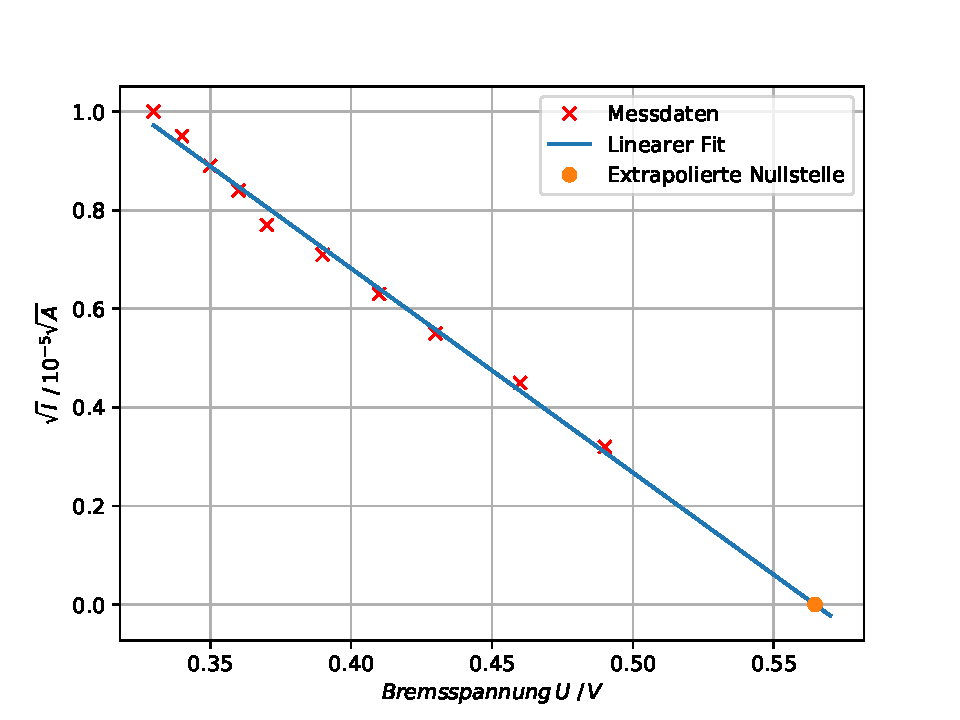
\includegraphics[width=0.8\linewidth]{LinieORANGE.pdf}
	\caption{Ausgleichsgerade zur Bestimmung der Grenzspannung bei $\lambda = 557\,\symup{nm}$.}
	\label{fig:orange}
\end{figure}

\begin{equation*}
\begin{aligned}
\lambda = 557\,\symup{nm} \text{:} \,\, a &=  (4{,}14 \pm 0{,}13)\cdot 10^{-5}\, \frac{\symup{A}^{\frac{1}{2}}}{V}\\
b &= (2{,}34 \pm 0{,}05)\cdot 10^{-5}\, \symup{A}^{\frac{1}{2}}\\ 
\end{aligned}
\end{equation*}

Da es sich bei $a$ und $b$ um fehlerbehaftete Größen handelt, muss der Fehlers von $U_{\text{g}}$ über die Gaußsche Fehlerfortpflanzung berechnet werden.

\begin{equation}
\begin{aligned}
\Delta{U}_{\text{g}} &= \sqrt{\biggl(\frac{\partial{U_{\text{g}}}}{\partial{b}}\biggr)^2 \cdot (\Delta b)^2+ \biggl(\frac{\partial{U_{\text{g}}}}{\partial{a}}\biggr)^2 \cdot (\Delta a)^2} \\
                     &= \sqrt{\frac{1}{a^2}\cdot (\Delta b)^2 + \frac{b^2}{a^4}\cdot (\Delta a)^2} \\
					 &= \sqrt{\frac{(\Delta b)^2 \cdot a^2 + b^2 \cdot (\Delta a)^2}{a^4}}
\label{eqn:fehlergrenzspannung}					 
\end{aligned}
\end{equation}
Werden $a$ und $b$ sowie deren Fehlerwerte in die Gleichungen \ref{eqn:grenzspannung} und \ref{eqn:fehlergrenzspannung} eingesetzt, so ergibt sich für die gesuchte Grenzspannung der Linie der Wellenlänge $\lambda = 557\,\symup{nm}$:

\begin{equation*}
U_{\text{g,\,557\,nm}} = (0{,}57 \pm 0{,}02)\,\symup{V}
\end{equation*}
Analog können so auch die Grenzspannungen der anderen Linien berechnet werden.



\newpage
\begin{table}[htbp]
\centering
\caption{Messwerte bei $\lambda = 546\,\symup{nm}$.}
\label{tab:some_data}
\begin{tabular}{S[table-format=1.2] S S S}
\toprule
{$U/ \, \symup{V}$} & {$I/10^{-9}\, \symup{A}$} & {$\sqrt{I}/\, 10^{-5}\symup{A^{\frac{1}{2}}}$} \\
\midrule
0.64 & 0.01 & 0.32 \\
0.61 & 0.02 & 0.45 \\
0.59 & 0.03 & 0.55 \\
0.57 & 0.04 & 0.63 \\
0.55 & 0.05 & 0.71 \\
0.54 & 0.06 & 0.77 \\
0.52 & 0.07 & 0.84 \\
0.51 & 0.08 & 0.89 \\
0.50 & 0.09 & 0.95 \\
0.49 & 0.1 & 1 \\
\bottomrule
\end{tabular}
\end{table}

\begin{figure}[h!tbp]
	\centering
	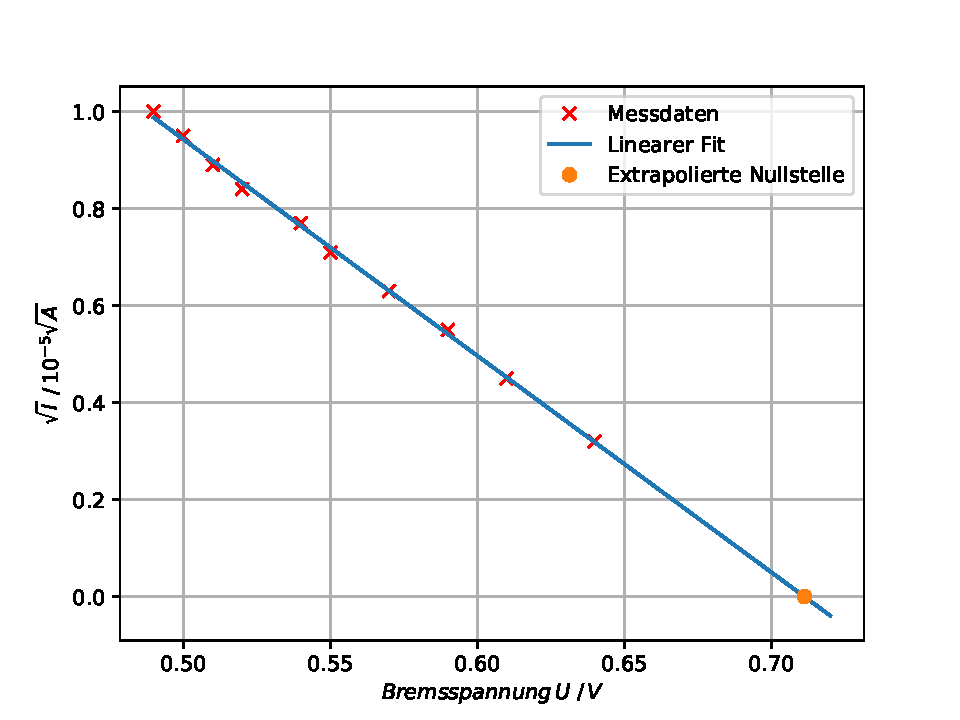
\includegraphics[width=0.9\linewidth]{LinieGRUEN.pdf}
	\caption{Ausgleichsgerade zur Bestimmung der Grenzspannung bei $\lambda = 546\,\symup{nm}$.}
	\label{fig:gruen}
\end{figure}

\begin{equation*}
\begin{aligned}
\lambda = 546\,\symup{nm} \text{:}\,\, a &=  (4{,}46 \pm 0{,}06)\cdot 10^{-5}\, \frac{\symup{A}^{\frac{1}{2}}}{V}\\
b &= (3{,}18 \pm 0{,}03)\cdot 10^{-5}\, \symup{A}^{\frac{1}{2}}\\ 
\implies U_{\text{g,\,546\,nm}} &= (0{,}71 \pm 0{,}01)\,\symup{V}
\end{aligned}
\end{equation*}



\begin{table}[htbp]
\centering
\caption{Messwerte bei $\lambda = 491{,}6\,\symup{nm}$.}
\label{tab:some_data}
\begin{tabular}{S[table-format=1.2] S S S}
\toprule
{$U/ \, \symup{V}$} & {$I/10^{-9}\, \symup{A}$} & {$\sqrt{I}/\, 10^{-5}\symup{A^{\frac{1}{2}}}$} \\
\midrule
0.54 & 0.01 & 0.32 \\
0.39 & 0.02 & 0.45 \\
0.23 & 0.03 & 0.55 \\
0.08 & 0.04 & 0.63 \\
0.11 & 0.05 & 0.71 \\
\bottomrule
\end{tabular}
\end{table}

\begin{figure}[h!tbp]
	\centering
	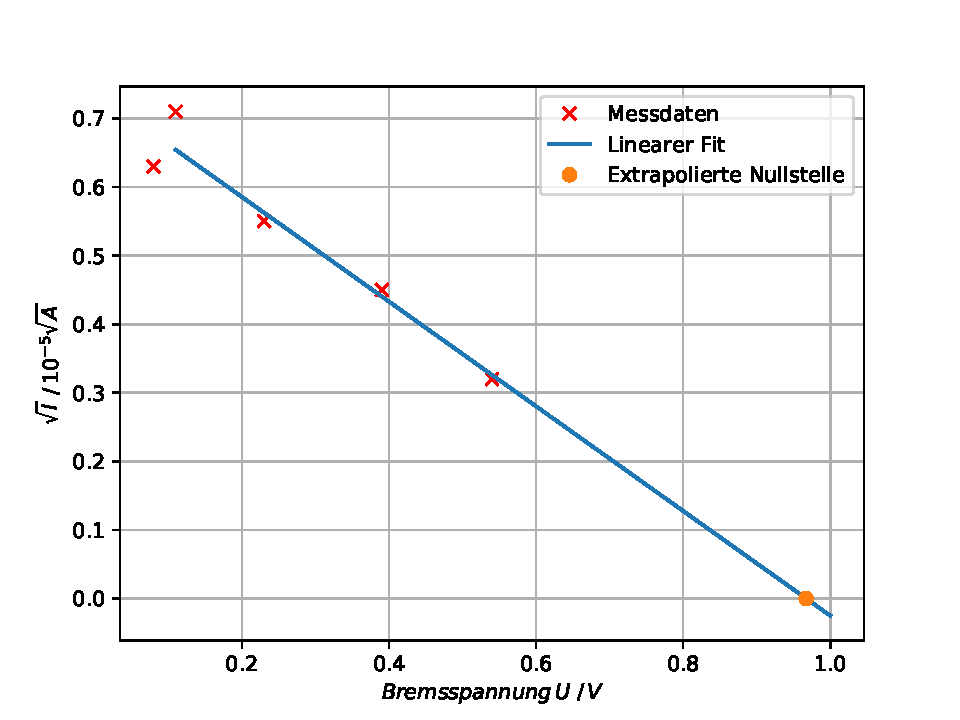
\includegraphics[width=0.9\linewidth]{LinieCYAN.pdf}
	\caption{Ausgleichsgerade zur Bestimmung der Grenzspannung bei $\lambda = 491{,}6\,\symup{nm}$.}
	\label{fig:cyan}
\end{figure}

\begin{equation*}
\begin{aligned}
\lambda = 491{,}6\,\symup{nm}\text{:}\,\, a &=  (0{,}763 \pm 0{,}112)\cdot 10^{-5}\, \frac{\symup{A}^{\frac{1}{2}}}{V}\\
b &= (0{,}74 \pm 0{,}04)\cdot 10^{-5}\, \symup{A}^{\frac{1}{2}}\\ 
\implies U_{\text{g,\,491,6\,nm}} &= (0{,}96 \pm 0{,}15)\,\symup{V}
\end{aligned}
\end{equation*}

\newpage

\begin{table}[htbp]
\centering
\caption{Messwerte bei $\lambda = 435{,}8\,\symup{nm}$.}
\label{tab:some_data}
\begin{tabular}{S[table-format=1.2] S S S}
\toprule
{$U/ \, \symup{V}$} & {$I/10^{-9}\, \symup{A}$} & {$\sqrt{I}/\, 10^{-5}\symup{A^{\frac{1}{2}}}$} \\
\midrule
1.16 & 0.01 & 0.32 \\
1.12 & 0.02 & 0.45 \\
1.08 & 0.03 & 0.55 \\
1.05 & 0.04 & 0.63 \\
1.03 & 0.05 & 0.71 \\
1.01 & 0.06 & 0.77 \\
0.98 & 0.07 & 0.84 \\
0.97 & 0.08 & 0.89 \\
0.96 & 0.09 & 0.95 \\
0.93 & 0.1 & 1 \\
\bottomrule
\end{tabular}
\end{table}

\begin{figure}[h!tbp]
	\centering
	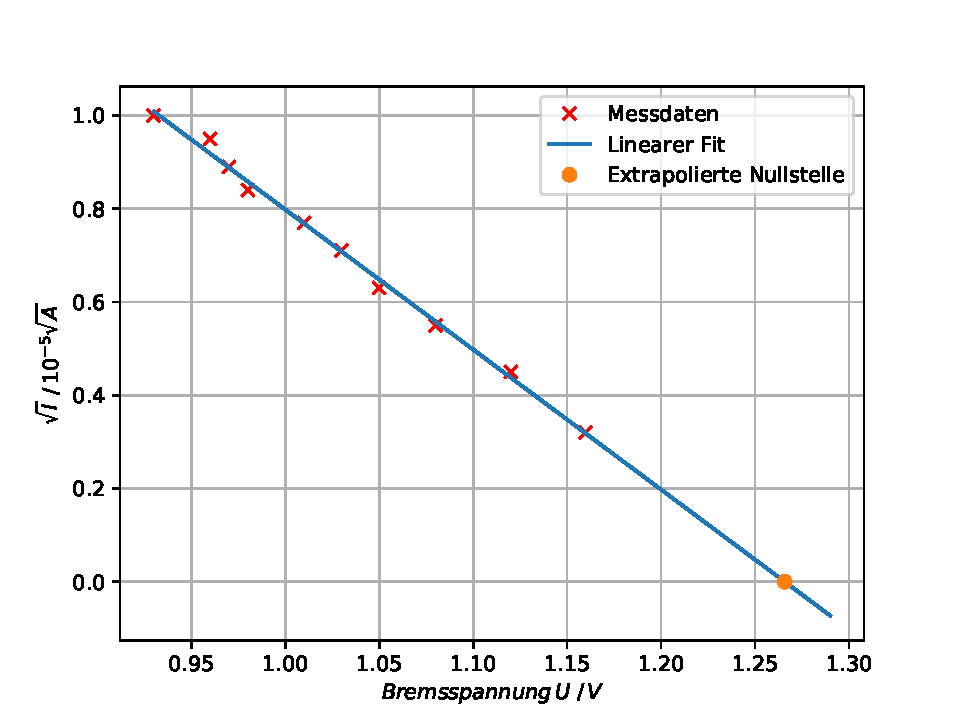
\includegraphics[width=0.9\linewidth]{LinieVIOLETT1.pdf}
	\caption{Ausgleichsgerade zur Bestimmung der Grenzspannung bei $\lambda = 435{,}8\,\symup{nm}$.}
	\label{fig:violett1}
\end{figure}

\begin{equation*}
\begin{aligned}
\lambda = 435{,}8\,\symup{nm}\text{:}\,\, a &= ({3,}00 \pm 0{,}07)\cdot 10^{-5}\, \frac{\symup{A}^{\frac{1}{2}}}{V}\\
b &= (3{,}80 \pm 0{,}07)\cdot 10^{-5}\, \symup{A}^{\frac{1}{2}}\\ 
\implies U_{\text{g,\,435,8\,nm}} &= (1{,}27 \pm 0{,}04)\,\symup{V}
\end{aligned}
\end{equation*}



\begin{table}[htbp]
\centering
\caption{Messwerte bei $\lambda = 407{,}8\,\symup{nm}$.}
\label{tab:some_data}
\begin{tabular}{S[table-format=1.2] S S S}
\toprule
{$U/ \, \symup{V}$} & {$I/10^{-9}\, \symup{A}$} & {$\sqrt{I}/\, 10^{-5}\symup{A^{\frac{1}{2}}}$} \\
\midrule
1.33 & 0.01 & 0.32 \\
1.27 & 0.02 & 0.45 \\
1.22 & 0.03 & 0.55 \\
1.19 & 0.04 & 0.63 \\
1.15 & 0.05 & 0.71 \\
1.13 & 0.06 & 0.77 \\
1.10 & 0.07 & 0.84 \\
1.08 & 0.08 & 0.89 \\
1.06 & 0.09 & 0.95 \\
1.03 & 0.1 & 1 \\
\bottomrule
\end{tabular}
\end{table}

\begin{figure}[h!tbp]
	\centering
	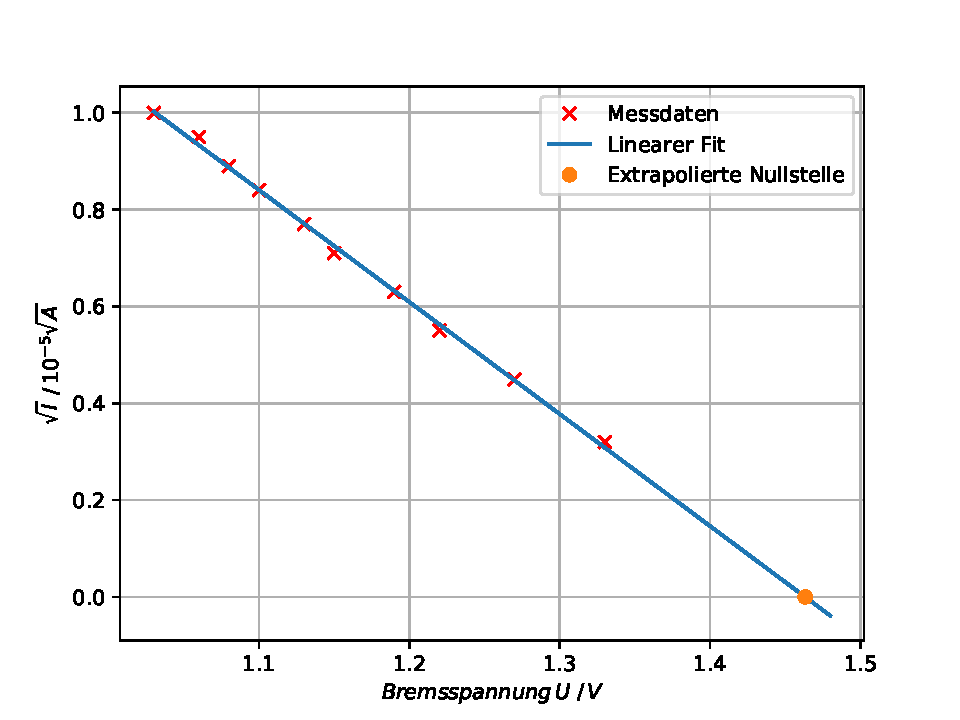
\includegraphics[width=0.9\linewidth]{LinieVIOLETT2.pdf}
	\caption{Ausgleichsgerade zur Bestimmung der Grenzspannung bei $\lambda = 407{,}8\,\symup{nm}$.}
	\label{fig:violett2}
\end{figure}

\begin{equation*}
\begin{aligned}
\lambda = 407{,}8\,\symup{nm} \text{:}\,\, a &= (2{,}31 \pm 0{,}04)\cdot 10^{-5}\, \frac{\symup{A}^{\frac{1}{2}}}{V}\\
b &= (3{,}39 \pm 0{,}04)\cdot 10^{-5}\, \symup{A}^{\frac{1}{2}}\\ 
\implies U_{\text{g,\,407,8\,nm}} &= (1{,}47 \pm 0{,}03)\,\symup{V}
\end{aligned}
\end{equation*}









\subsection{Bestimmung des Verhältnisses $\frac{h}{e_0}$ und der Austrittsarbeit $A_{\text{K}}$}

Um das Verhältnis $\frac{h}{e_0}$ und die Austrittsarbeit $A_{\text{K}}$ zu bestimmen, müssen die berechneten Gegenspannungen $U_{\text{g}}$ gegen die Lichtfrequenzen $\nu$ aufgetragen werden.
Zu finden sind diese in Tabelle \ref{tab:verhaeltnis}. Die Wellenlängen werden aus den Versuchsunterlagen entnommen. Die Umrechnung von Wellenlänge in Frequenz geschieht über die 
Lichtgeschwindigkeit $c = 299792458\, \symup{\frac{m}{s}}$:

\begin{equation}
\nu = \frac{c}{\lambda}.
\end{equation}

\begin{table}[htbp]
\centering
\caption{Messwerte zur Bestimmung von $\frac{h}{e_0}$ und $A_{\text{K}}$. }
\label{tab:verhaeltnis}
\begin{tabular}{S[table-format=1.4, table-figures-uncertainty=1] S[table-format=3.1] S[table-format=3.2] }
\toprule
{$U_{\text{g}}/ \, \symup{V}$} & {$\lambda/10^{-9}\, \symup{m}$} & {$\nu/\, 10^{12}\symup{Hz}$} \\
\midrule
0.57 \pm 0.02     & 557.0 & 538.23 \\
0.71 \pm 0.01     & 546.0 & 549.07 \\
0.96 \pm 0.15     & 491.6 & 609.83 \\
1.27 \pm 0.04     & 435.8 & 687.91 \\
1.47 \pm 0.03     & 407.8 & 735.15 \\

\bottomrule
\end{tabular}
\end{table}

\begin{figure}[h!tbp]
	\centering
	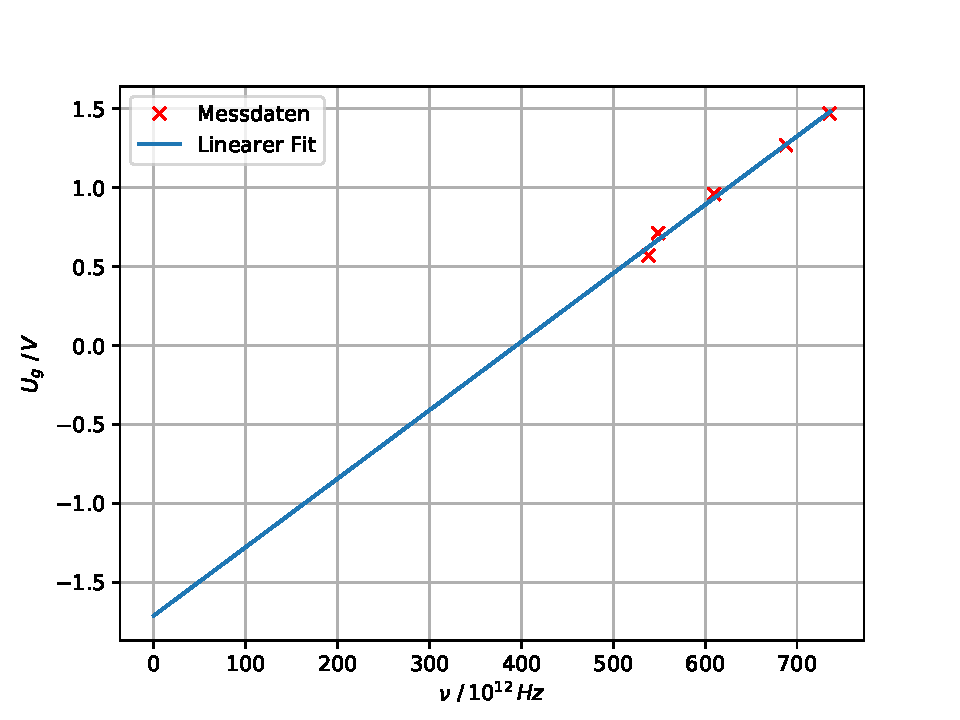
\includegraphics[width=0.8\linewidth]{verhaeltnis.pdf}
	\caption{Ausgleichsgerade zur Bestimmung des Verhältnisses $\frac{h}{e_0}$ und der Austrittsarbeit $A_{\text{K}}$.}
	\label{fig:verhaeltnis}
\end{figure}

\begin{figure}[h!tbp]
	\centering
	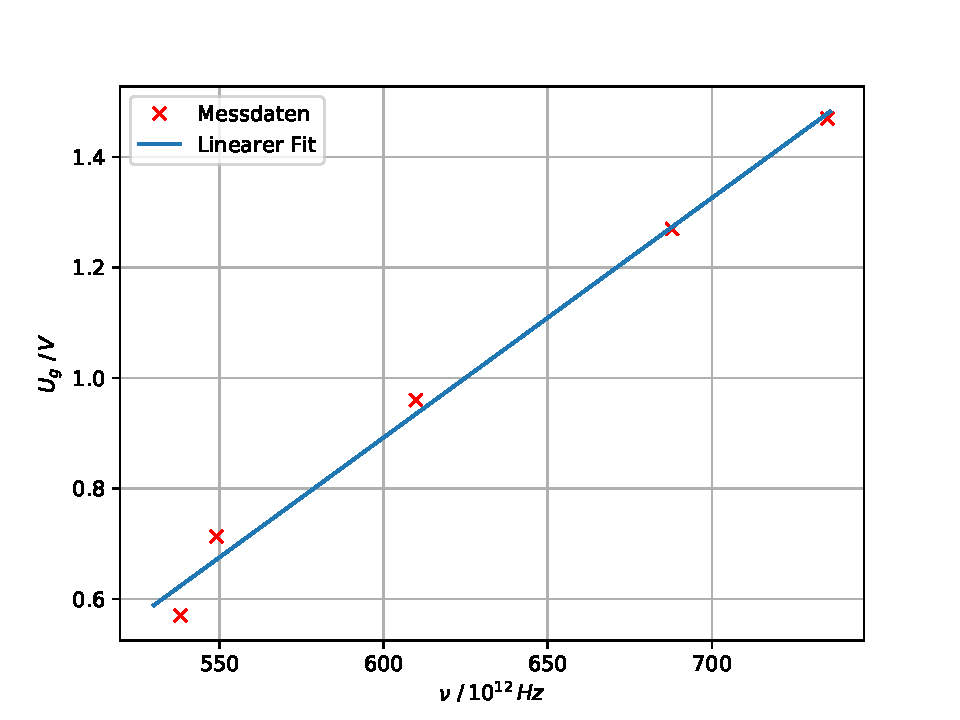
\includegraphics[width=0.8\linewidth]{verhaeltnis2.pdf}
	\caption{Ausgleichsgerade zur Bestimmung des Verhältnisses $\frac{h}{e_0}$ und der Austrittsarbeit $A_{\text{K}}$.}
	\label{fig:verhaeltnis}
\end{figure}


Nach Formel \ref{eq:eq3} ist das Verhältnis $\frac{h}{e_0}$ gleich der Steigung der Ausgleichsgeraden, die Austrittsarbeit $A_{\text{K}}$ entspricht dem Y-Achsenabschnitt. Mithilfe von Scipy curve-fit werden diese zu

\begin{equation*}
\begin{aligned}
\frac{h}{e_0} &= (4{,}3 \pm 0{,}2 )\cdot 10^{-15}\, \symup{\frac{Js}{C}} \\
A_{\text{K}} &= (1{,}71 \pm 0{,}15)\, \symup{eV}
\end{aligned}
\end{equation*}
bestimmt.




\subsection{Untersuchung des Photostroms bei Licht der Wellenlänge \texorpdfstring{$\lambda = 578\,\symup{nm}$}{Lambda = 578\,nm}.}
Zuletzt wird der Photostrom von gelben Licht der Wellenlänge $\lambda = 578\,\symup{nm}$ in Abhängigkeit von der Spannung, welche in einem Intervall von $-20\,\symup{V}$ bis $20\,\symup{V}$ eingestellt werden soll, untersucht. Die Messwerte sind in Tabelle \ref{tab:orangePhoto} zu finden. 
Aufgetragen sind sie in Abbildung \ref{fig:orangePhoto}.
\begin{table}[htbp]
\centering
\caption{Messwerte zur Untersuchung des Photostroms bei $\lambda = 578\,\symup{nm}$.}
\label{tab:orangePhoto}
\begin{tabular}{S[table-format=2.2] S[table-format=2.3] S[table-format=2.2] S[table-format=2.3]  }
\toprule
{$U/ \, \symup{V}$} & {$I/10^{-9}\, \symup{A}$} & {$U/ \, \symup{V}$} & {$I/10^{-9}\, \symup{A}$} \\
\midrule
-19.15 & 2.597 & -4.00 & 1.465 \\
-18.01 & 2.513 & -3.00 & 1.265\\
-17.00 & 2.460 & -2.00 & 0.932\\
-16.00 & 2.397 & -1.80 & 0.965\\
-15.00 & 2.331 & -1.60 & 0.799\\
-14.00 & 2.264 &-1.40 & 0.732 \\
-13.00 & 2.231 & -1.20 & 0.666\\
-12.00 & 2.164 & -1.00 & 0.666\\
-11.00 & 1.998 & -0.80 & 0.561\\
-10.00 & 1.964 & -0.60 & 0.533 \\
-9.00 & 1.898  & -0.40 & 0.466\\
-8.00 & 1.731  & -0.20 & 0.399\\
-7.00 & 1.665  & 0.00  & 0.266\\
-6.00 & 1.598  & 0.2  & 0.133 \\
-5.00 & 1.531  & 0.4  & 0.226\\


\bottomrule
\end{tabular}
\end{table}


\begin{figure}[h!tbp]
	\centering
	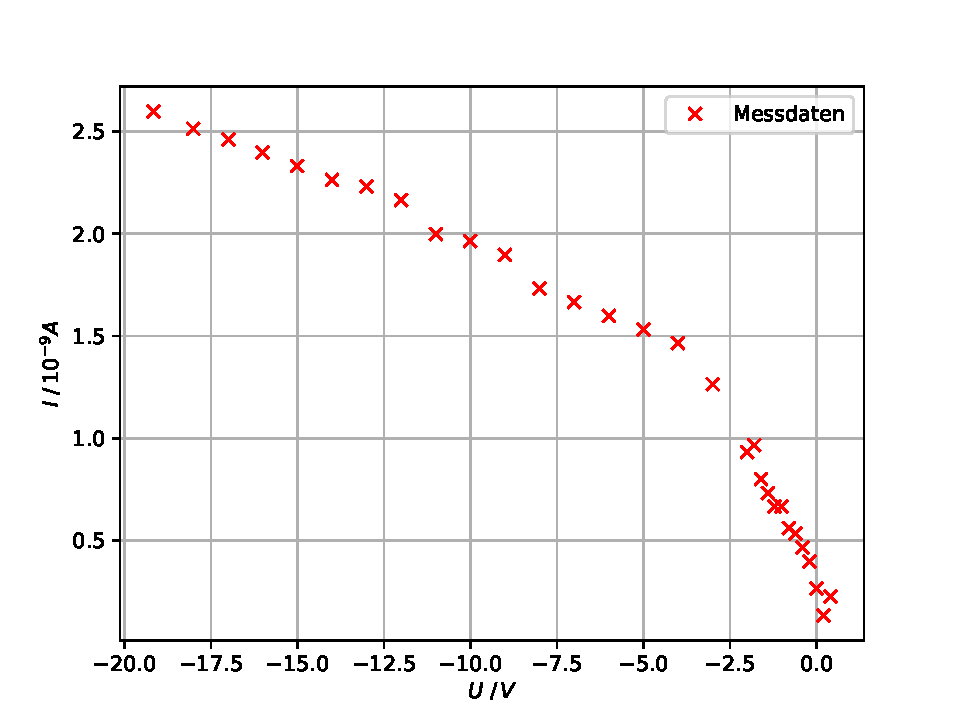
\includegraphics[width=0.8\linewidth]{orangePhoto.pdf}
	\caption{Verlauf des Photostroms in Abhängigkeit der Spannung bei $\lambda = 578\,\symup{nm}$.}
	\label{fig:orangePhoto}
\end{figure}
Wie in Abbildung \ref{fig:orangePhoto} zu erkennen ist, geht der Photostrom für hohe Beschleunigungsspannungen gegen einen Sättigungswert. Grund dafür ist, dass es auf der Kathode nur endlich viele Elektronen gibt, die heraustreten können.
Würden all diese durch die Beschleunigungsspannung zur Anode wandern, würde sich ein Sättigungswert einstellen, der von der Anzahl der Elektronen abhängt, welche wiederum auch mit der Lichtintensität zusammenhängt. In der Praxis wird dieser Sättigungswert 
allerdings nur asymptotisch erreicht, da wegen der kleineren Fläche der Anode nicht alle Elektronen auftreffen. Hier könnte also beispielsweise eine größere Anode eingesetzt werden, damit mehr Elektronen zum Photostrom beitragen können.
Es fällt ebenso auf, dass der Photostrom schon für Spannungen fällt, die kleiner sind als die Grenzspannung. Dies lässt sich mit der Fermi-Dirac-Verteilung erklären. Die Elektronen in der Kathode besitzen unterschiedliche Energien, woraus folgt, dass 
es auch bei einer einheitlichen Lichteinstrahlung eine Energieverteilung der ausgetretenen Elektronen gibt. Somit bricht der Photostrom mit einer bestimmten Grenzspannung nicht abrupt ab, weil es auch energiereichere Elektronen gibt, die eine höhere 
Bremsspannungen benötigen und ebenso gibt es energieärmere Elektronen, die schon bei geringen Bremsspannungen nicht die Anode erreichen.

Beim Photoeffekt ist es möglich, einen negativen Photostrom zu erreichen. Da das Material der Kathode schon bei 20°C verdampft und sich auf der Anode absetzt, kann auch dort der Photoeffekt stattfinden. Auf diese Weise würden bei einer angelegten 
Bremsspannung Elektronen aus der Anode zur Kathode wandern und so einen negativen Photostrom bewirken. Da die Anzahl der Elektronen in diesem Fall aber geringer ist, wird der Sättigungswert schneller erreicht. Die Tatsache, dass schon energiearmes Licht 
einen solchen Photostrom auslöst spricht dafür, dass die Anode eine geringe Austrittsarbeit besitzt, sodass die Elektronen leicht austreten können.